
\chapter{Water - Benthic Interface}
\chapterauthor{Alison Hong and Sami Murphy}

\section{Introduction}  
The lowest layer of a body of water, the benthic layer, is a fascinating and highly productive ecological region that interacts with nearby sediments, chemical elements, and organisms. In coastal waters, the benthic zone facilitates nutrient and biogeochemical processes that sustain a significant amount of biodiversity. Without this water layer, lakes, rivers, and oceans, among many other types of bodies of water, would not be able to support benthic aquatic life.

In this bottom-most layer of water, biotic (living) and abiotic (non-living) members of the benthic community facilitate vertical processes. The benthic zone is vital to aquatic ecosystems by providing an interface for sediment exchanges and oxygenation (dissolved oxygen in water). Basic roles like nutrient cycling and contaminant filtration need to be maintained, or natural catastrophes like sea level rise, coral reef degradation, and coastal village collapse can occur. In this chapter, we will explore the interactions that take place in benthic regions, focusing on the relationships between soil, water, land, and aquatic life. To understand the productivity and importance of the rhizosphere (the region of soil directly influenced by root secretion and microorganisms) and benthos, we will use Southeast Asian mangroves as a model. Mangrove efficiency outputs are vital to the viability and sustainability of aquatic ecosystems. 

%\section{Southeast Asia}
%Southeast Asia is an incredibly diverse part of the world that is comprised of countries of varied geography, weather, and environmental conditions. Temparate and tropical weather conditions provide ideal circumstances for luscious vegetation. The countries in Southeast Asia are major exporters for crops such as rice, cotton, and soybeans, amongst many others.

\section{Benthos: A Critical Ecological Value}

As the lowest layer of a body of water, the benthic layer serves as a foundation for many ecosystems. Located directly above the sediment in a river, lake, or sea, it is the site for nutrient exchanges and metabolic processes. The organisms that reside on the benthic layer are called benthos. Benthos are abundant in shallow waters off the coast, which makes Southeast Asia an ideal environment for benthos to reside. Benthos in Southeast Asia are found in estuaries, mangrove farms, and rivers.

\begin{figure}[!h]
        \centering
        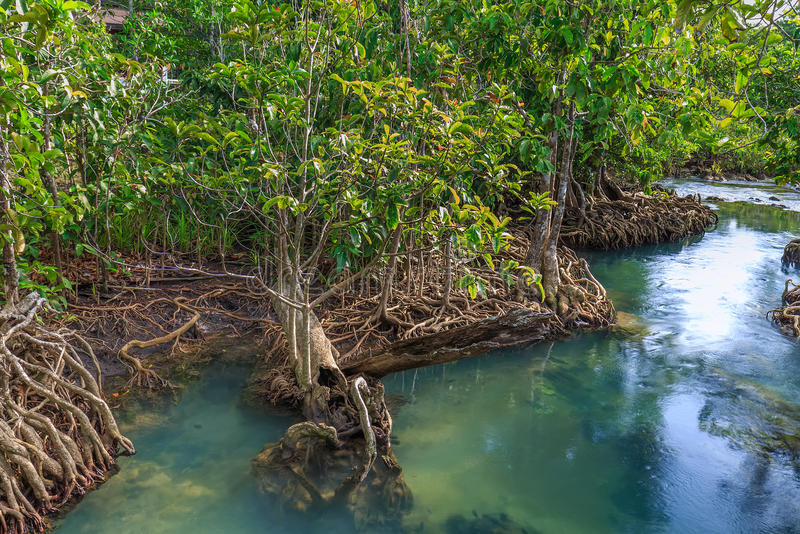
\includegraphics[width=4in]{mangrove.jpg}
        \caption{Mangrove Forest in Thailand}
        \label{fig:Benthos Mangroves in Thailand}
\end{figure}

\subsection{Oxygen in the Atmosphere}
Oxygen is abundant in earth, making up about 21\% of the atmosphere. During the Great Oxygenation Event 2.4 billion years ago, many anaerobic organisms became extinct due to the high amount of free oxygen in earth's atmosphere. Today, aerobic species and organisms are able to thrive with earth's large supply of free atmospheric oxygen. Oxygen is the most abundant chemical element in the earth's biosphere and serves as the foundation for many biological pathways and processes. It is produced during photosynthesis and used in mitochondria to drive the production of ATP. Oxygen is not only present in the atmosphere, but also available in water, as dissolved oxygen (DO).

\subsubsection{Reduced Availabilty of Oxygen in Water}
When oxygen enters water, a diffusion barrier exists between the air and the water. Because water does not have the ability to hold as much oxygen as the atmosphere due to its crystyalline structure, there is a much lower concentration of oxygen in water compared to in the air. Compared to the 21\% of oxygen in the atmosphere, it makes up less the 1\% of the ocean's composition. When the two surfaces meet, oxygen in the air dissolves into the the water. As natural forces move the water, such as wind and current, oxygen dissolves at a higher rate. Dissolved oxygen rates depend on the temperature and salinity of water. Cold waters contain more dissolved oxygen than warm waters and fresh waters can hold more than salt waters. Thus, cold fresh waters are the bodies of water that contain the most DO. 

\subsubsection{Dissolved Oxygen and Decomposition}
Oxygen plays a major role in the breakdown of organic matter. When organic matter falls to the benthic layer of a body of water, it is decomposed by bacteria that uses oxygen during aerobic decomposition processes. However, when the bacteria consumes all the DO available in the water, aerobic decomposition processes begin to occur at a much lower rate, because of the lack of DO. As a result, water become stratified because the DO from the top layer does not dissolve with other water layers and an imbalance of DO results. This phenomenon is called density stratification. Density stratification occurs in costal systems dominated by waves and results from low levels of tidal mixing when freshwater with low salinity flows over denser marine waters with higher salinity levels. The barriers created by the disproportion of DO levels disallow nutrients to flow within the different water layers and photosynthetic processes can be limited. The bottom water layer becomes anoxic, meaning there is a lack of oxygen. Thermal statification can also occur in waters. In a thermally stratified lake, the densest layer, the hypolimnic layer, remains cold during the summers and warm during winters. During summer, when the surface water is warmed by the sun, cooler water separate and two layers that differ in density are formed. Additionally, hypolimnetic DO in eutrophic lakes declines in the summer because there is no source of oxygen; however, the benthic organisms continue to consume oxygen (eutrophy refers to the most productive stage of a lake's life). As a result of the continued demand for oxygen but lack thereof, benthic organisms are not able to resume their aerobic processes. 


\begin{figure}[!ht]
        \centering
        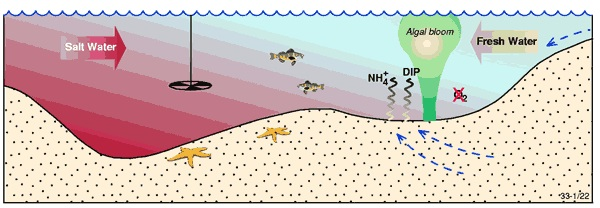
\includegraphics[width=4in]{salinitynew.jpg}
        \caption{Saline stratification in marine waters}
        \label{fig:Salinity}
\end{figure}


\begin{figure}[!ht]
        \centering
        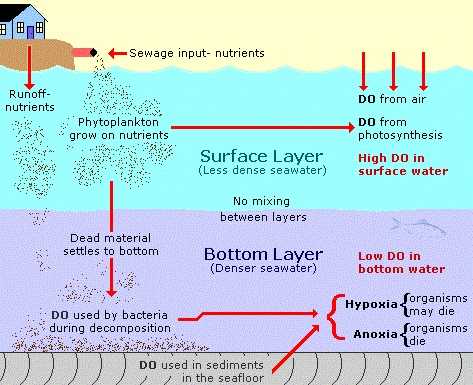
\includegraphics[width=4in]{water_oxygen.jpg}
        \caption{Dissolved Oxygen Levels in Water}
        \label{fig:DO Levels}
\end{figure}

\subsubsection{How do benthic animals respond in anerobic environments?}
Since anoxia is a seasonal process, benthic animals have anticipated responses to low oxygen rates. When an absence of oxygen exists in the benthic level, benthos respond by surfacing out of their habitats within the benthic sediment. The organismal beds that result further deplete the available oxygen level in the benthic layer \citep{jorgensen1980seasonal}. The layer becomes stagnant as a result from the oxygen deficiency and sparks anaerobic metabolic processes. As a result, the product of sulfate reduction, hydrogen sulfide, accumulates from the anaeorbic processes. Sulfate reduction will further be discussed in an upcoming section.

Reading Activity: Discuss with a friend other ways you think animals respond to a lack of available oxygen.

\section{Biogeochemistry}
\subsection{Sediment-Water Interface}

The sediment-water interface includes interactions between the benthic water layer and upper region of the sediment bed. Benthic cycling of nutrients and metals occurs at this interface. This layer can includes detrital material (weathered rock fragments) that contain aggregates that have deposited from higher water levels \citep{turley2000bacteria}. This sediment is involved with oxidation and reduction processes facilitated by bacteria.
Approximately 75\% of bacterial biomass in waters is found in the top 10 cm of sediments. Additionally, bacteria in oceanic and coastal sediments make up 76\% of the Earth's bacteria \citep{turley2000bacteria}. 

\begin{figure}[!h]
        \centering
        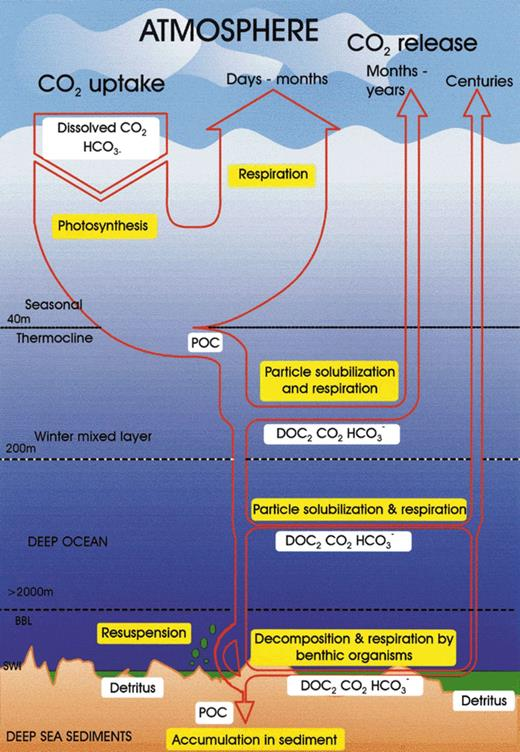
\includegraphics[width=3in]{sediment_water.jpg}
        \caption{Chemical Transfers in Sediment-Water Interface}
        \label{fig:Sediment-Water Processes}
\end{figure}

\subsection{Nutrient Cycling}
The abundance of certain minerals varies seasonally due to the availability of oxygen and organic material \citep{friedrich2002benthic}. Oxygen concentrations change considerably throughout the year and can vary in and off shore. In near-shore ecosystems, the primary site of mineralization occurs within sediment. Depending on how organic matter settles on sediments and if they are impacted by bioturbation (the reworking of sediments and soils by organisms), organic matter will be classified into either oxic or anoxic zones. In these zones, bacteria processes mineralize the matter \citep{spooner2009benthic}. The water is then able to provide elements such as oxygen, calcium, and sodium to benthic organisms.

\subsection{Benthic Metabolism}

Both organic and inorganic compounds travel through the vertical interface between the benthic and rhizospheric zones. Abiotic factors within the benthic layer, such as water temperatures, DO, light, and sediments, help process nutrients in the benthic water layer. Sulfate reduction and carbon cycling are examples of cycles and processes that help break down nutrients on the benthic level that provide sustenance for various ecosystems. In Thai mangroves, benthic metabolism influences the soil and nutrient-richness of the benthic-soil interface.

Reading Activity: What are some examples of biotic factor that help facilitate metabolic processes?

\subsubsection{Sulfate Reduction and Oxidation}
Sulfate reduction is an anaerobic respiration process that occurs in waters and sediments. It is facilitated by sulfate-reducing bacteria and archaea that aid in degradation (break-down) processes of organic materials. During the sulfate reduction process, sulfate acts as a terminal electron acceptor and is reduced to hydrogen sulfide. The resulting smaller compounds are further oxidized by methanogens, methane-producing microorganisms in anoxic conditions. Although hydrogen sulfide is a harmful substance to humans that can contaminate drinking water, it is environmentally beneficial and is used to convert contaminants such as uranium, chromium, and technetium from soluble to insoluble forms. 

Sulfate reduction is influenced by many factors, such as season, benthic community activity and physical transport conditions. It is vital to benthic water ecosystems and has been found to be responsible for up to all of the total benthic metabolism in highly productive and undisturbed coastal environments. It is responsible for 20-30\% of total carbon oxidation \citep{kristensen2000carbon}. This process is prevalent and vital to mangrove metabolism and chemical cycling. 




\subsubsection{Sulfate Reduction in Mangroves}
Mangrove swamps constantly degrade and recycle sediments into adjacent areas. The sulfate-reducing bacteria present in mangroves acts as a reducing agent during anaerobic respiration. Since organic matter is oxidized in the benthic sediment layer, sulfate-reducing bacteria is important in the mineralization of organic carbon. 


Organic detritus produced in mangrove swamps degrade and recycle sediments or export them into adjacent areas. Vertical translocation of metabolizable organic substrates, due to either subsurface root growth or due to downward transport of newly deposited organic matter by bioturbation are responsible for high subsurface activity. There are similar mechanisms observed in salt marshes \citep{kristensen1991benthic}.

\begin{figure}[!ht]
        \centering
        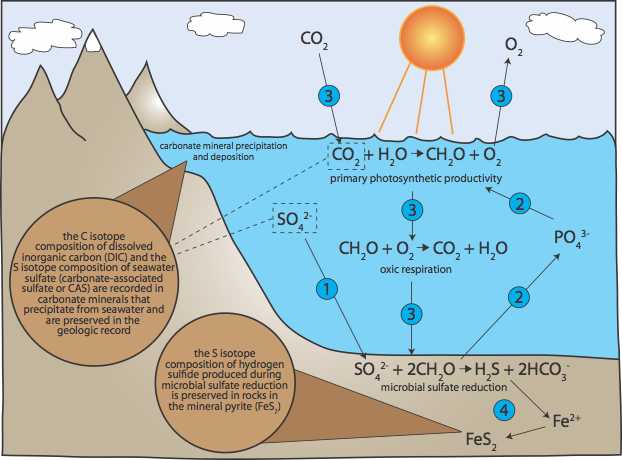
\includegraphics[width=3in]{sulfate_reduction.png}
        \caption{Sulfate Reduction Cycling}
        \label{fig:Sulfate Reduction}
\end{figure}



\subsubsection{Carbon Cycling}
Carbon cycling is prevalent in coastal waters, as the shallow waters allow primary producers to graze the bottom of the waters. Additionally, because light is able to reach the bottom waters, it is able to catalyze many chemical reactions. Typically, there is a higher percent of sediment organic carbon content in freshwater compared to ocean water. In the deep ocean, the benthic level occupies two thirds of the earth and provides a great deal of the carbon sequestration and regeneration of nutrients. When carbon dioxide enters the ocean surface during carbon dioxide exchanges with the atmosphere, it reacts with water to form the dissolved inorganic carbons, bicarbondate and carbonate ions. This inorganic carbon remains in ocean waters and can either be transformed into dissolved organic carbon or can be taken up by phytoplankton during photosynthesis. Carbon is cycled through different levels of the foodweb and from different layers of a body of water.  


\section{Mangroves}

\subsection{What are mangroves?}

  Mangroves are estruatrian trees that thrive along the coasts of tropical regions. Their salt tolerant, sturdy roots both protrude from the tree and are nestled deep within the ground. These roots, which are numerous and intertwined, are a defining physical characteristic of this species. In fact, \textit{Rhizophoraceae Rhizophora}, known as the �true mangrove� and most commonly found throughout Southeast Asia, is translated as roots (``rhiz") above ground (``phora"). Growing up to 25 meters tall, mangroves are thin and long in shape with dense leaves near their heads. Because these forests are often cluttered with overlapping trees, they are substantial barriers between oceanic waves and coastal communities. As they block external turbulence from the ocean from degrading the coastline, mangroves simultaneously protect the sea from inland pollutant runoff and heavy organic matter deposition.  As ecological filtration systems, they are vital to estuarine environments by mitigating toxic leakage from agrarian pesticides and fertilizers. In this chapter, the nutrient cycling and sequestration that takes place within mangroves will demonstrate the importance of benthos as foundations of wetland environments.




%\begin{figure}[!h]
% \centering
%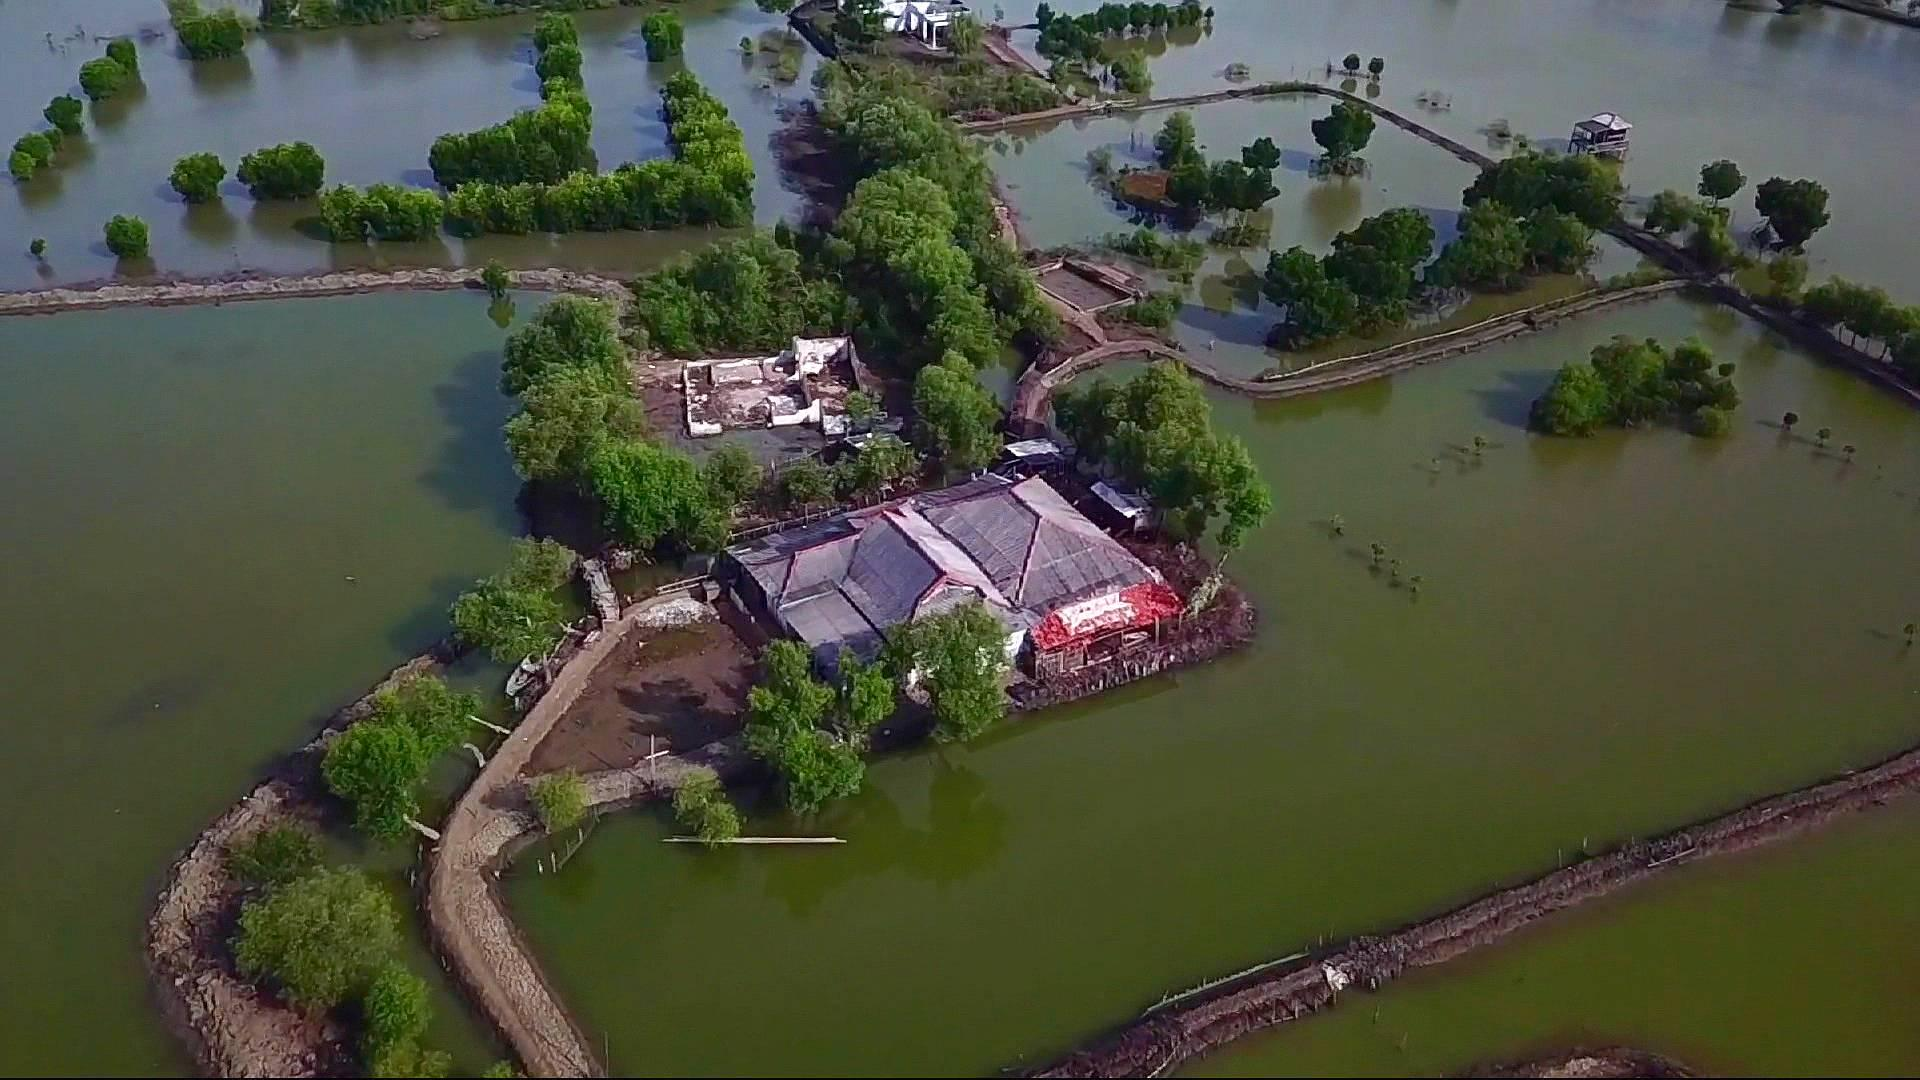
\includegraphics[width=3in]{flooded_village_indonesia.jpg}
% \caption {This is but one example of the many Indonesian and Southeast Asian coastal villages exposed to flooding due to sea level rise. Because flooding has escalted past the point of remediation (i.e. planting mangroves), the community must either adapt to life as a floating village or live elsewhere. In this case, members of the community wil probably leave their traditional lifestyles behind and seek work in more urban and inland cities.}
%   \label{fig:Bahagia_Village}
% \end{figure}
      
      
\subsection{Reproduction}

  Proper tidal currents, insects, and nutrient conditions must be met for mangrove reproduction to occur. If an environment hosts a good balance of these qualities, then seedling production and pollination may be facilitated.  In fact, without wind and insects, mangrove reproduction success rates may be as low as 11.48\%. Viviparous and crypto-viviparous species of mangrove are both self-pollinating and cross-pollinating, and their seeds are very large \cite{ge1999reproductive}. Viviparous species produce offspring that begin growth while still attached to the parent plant. Starting as a flower bud, it takes about four months to reach seedling size, yet this varies amongst mangrove species. Similar to fetuses during pregnancy, mangrove seedlings depend on their parent for nutrients and a safe environment to evolve in its initial stages of life. While in this primary phase, the seedling ``develops chlorophyll and actively photosynthesizes" as ``the parent tree supplies the water and necessary nutrients" \citep{selvam2004ecology}.  Toward the end of this process, ``the seedling hangs downward and detaches from the residual fruit at the collar end (base of branch where it connects to the trunk), leaving behind its cotyledons (embryonic leaves), and falls from the maternal parent", after about four to six months of maturation and begins growth as an independent organism . The process from seedling to towering canopy begins when the fully developed seedling implants itself into the mud either directly after detachment or after dispersal from oceanic tides \citep{aluri2013reproductive}. However, unruly tidal currents can make it difficult for seedlings to implant, animals such as crabs and monkeys may destroy vulnerable seedlings, and climate change can alter flowering patterns and schedules \citep{aluri2013reproductive}.

	It is important to understand the reproductive processes of mangroves as the vitality of entire ecosystems depends on the success of this regeneration. 
	
\begin{figure}[!htb]
      \centering
        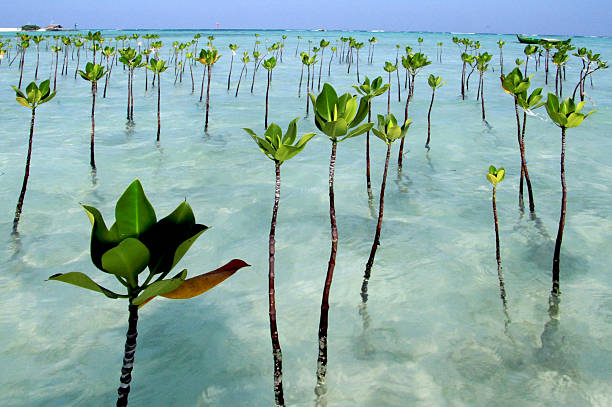
\includegraphics[width=3in]{growingmangrove.jpg}
        \caption {Stage 4: Growth from Seedling to a Tree}
        \label{fig:Mangrove_Stage4}
\end{figure}
      
\subsection{Tannin Value}

  While the roots of mangroves are important for nutrient cycling and soil anchoring, their trunks hold economic value in their bark. Fishermen find value in the tannin that gives the bark a reddish-brown color (figure \ref{fig:tannins}). With up to 68 to 78\% tannin concentrations, this bark contains reddish liquid that can be extracted and used to protect cotton fishing nets from decay for a longer period\citep{aluri2013reproductive}.


	Beyond this, tannins affect estuarine efficiency in mangroves, particularly because of their relationship to nitrogen. They are also suppliers of DOM (dissolved organic matter) and ``strong absorbers of light" due to their dark hue, which �facilitates photochemical reactivity" \citep{maie2008mangrove}. The most important role of tannins in estuarian environments however, lies within their ability to create ``stable tannin-protein complexes" that sequester nitrogen. In other words, they keeps nitrogen trapped within the benthic zone (figure \ref{fig:tannindiagram}. Nitrogen, a component of amino acids, is vital for the construction of proteins and thus, the formation of life. Without soil rich in nitrogen, biotic growth would not be possible. To simplify, the sequestration of DON (dissolved organic nitrogen) means the sequestration of proteins, which are the foundation of all living things.  
	
Reading Activity: From what you have read thus far, how are mangroves unique from other forest ecosystems? 


\begin{figure}[!htb]
      \centering
        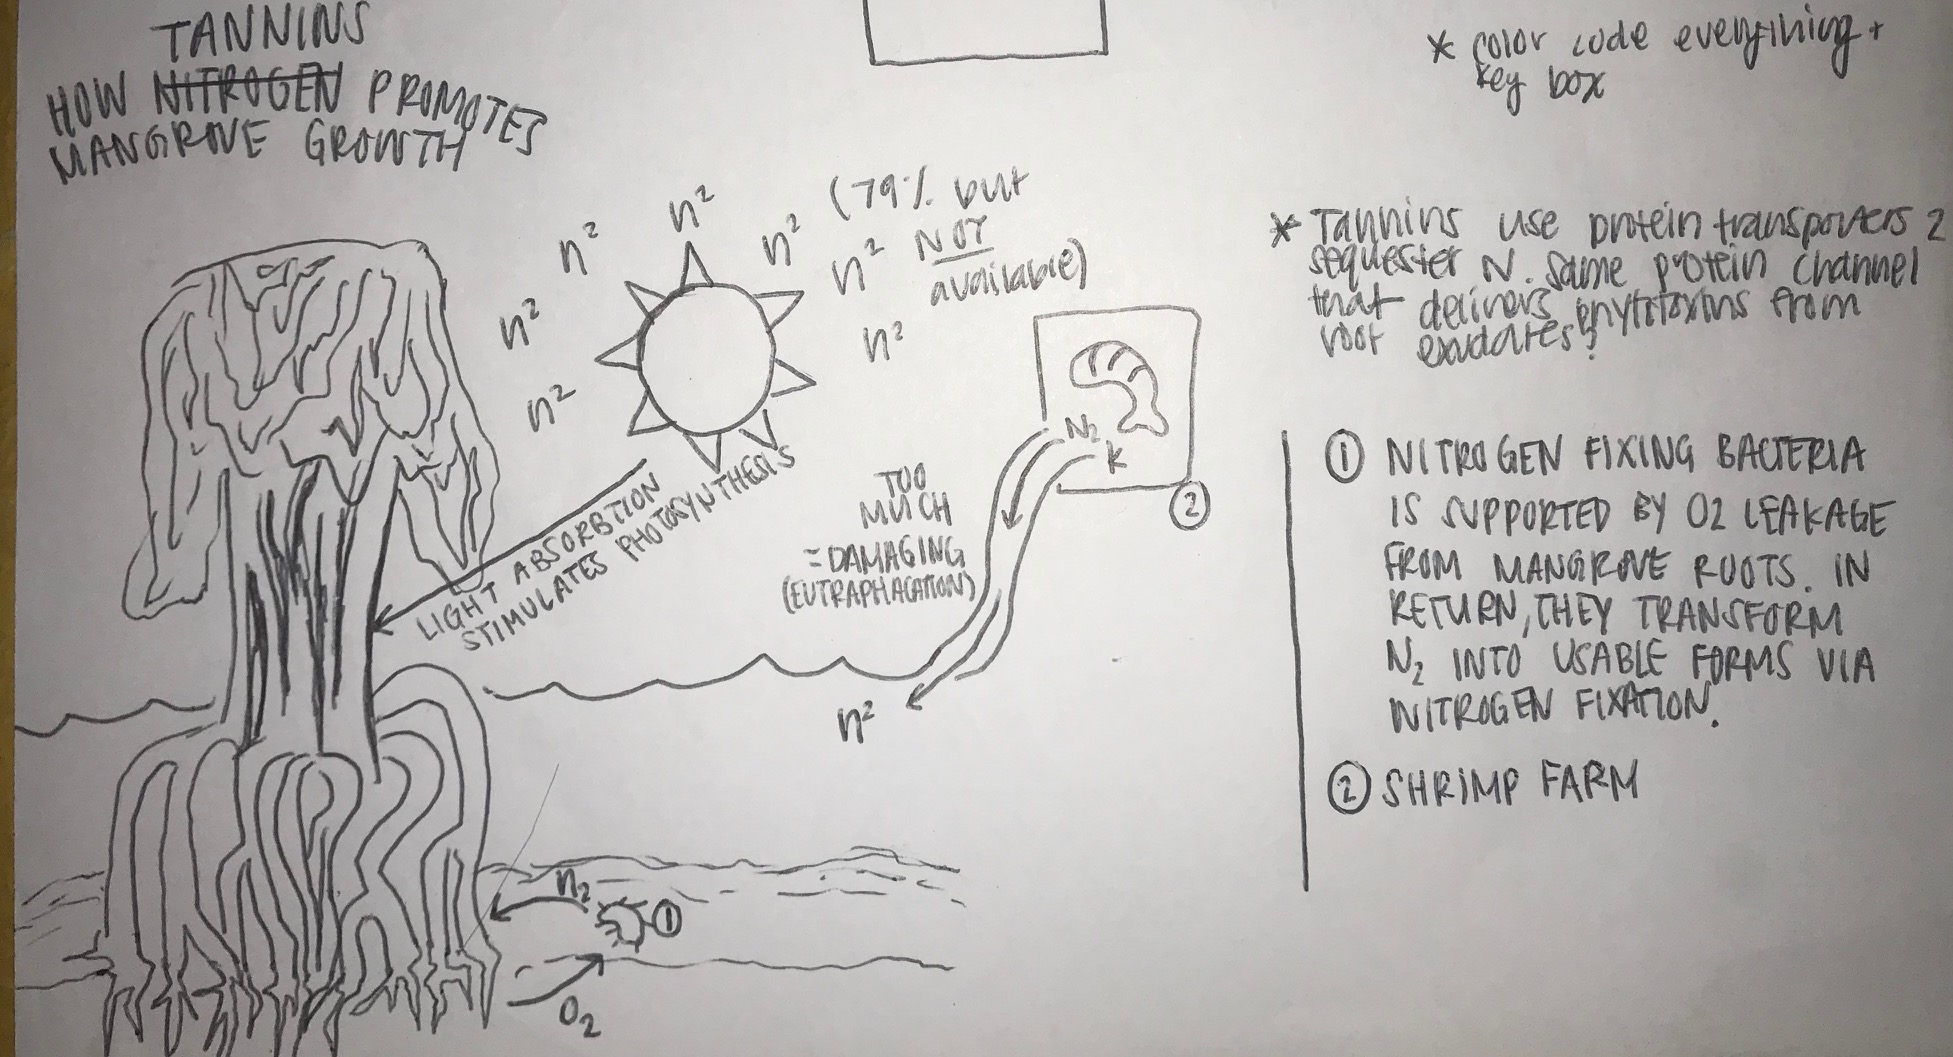
\includegraphics[width=4in]{tannindiagram.jpg}
        \caption {Tannins processes in mangroves}
        \label{fig:tannindiagram}
\end{figure}

\begin{figure}[!htb]
        \centering
        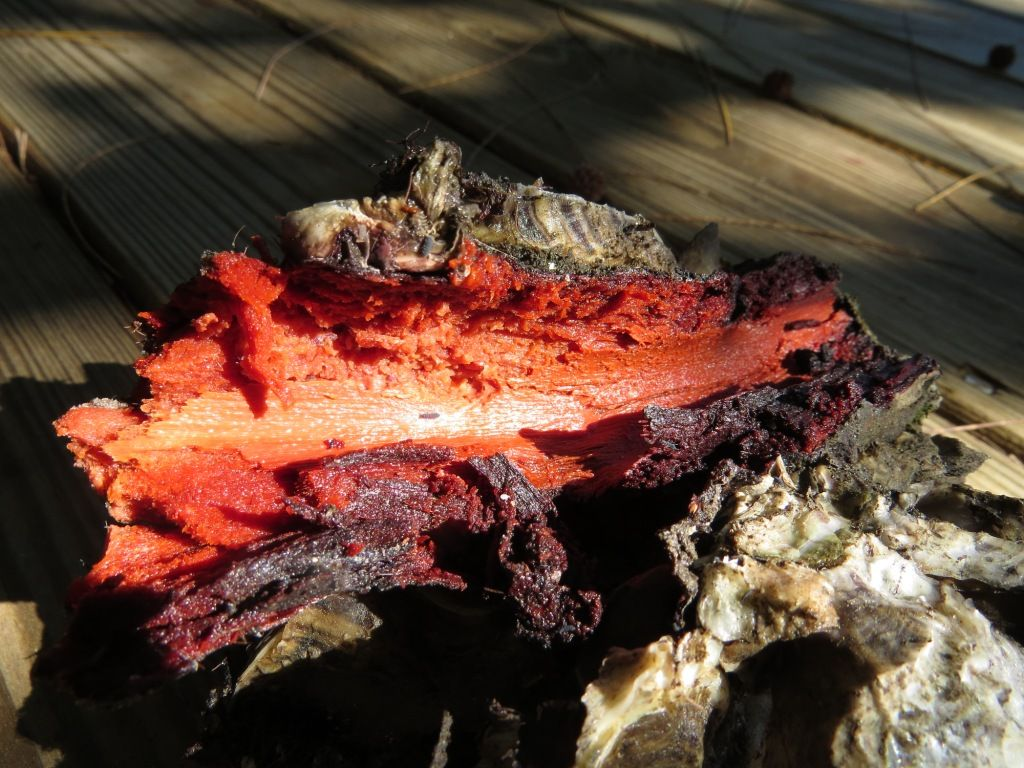
\includegraphics[width=2.5in]
        {tannins.jpg}
        \caption {Mangrove tannins: the reddish insides of mangrove bark are tannins. }
        \label{fig:tannins}
      \end{figure}


\subsection{The Ecological and Economic Importance of Mangroves}

\subsubsection{Environmental Benefits of Mangroves}
  Mangroves indirectly impact a variety of economic and ecological variables. Although degradation of mangroves cause many immediate problems to their specific estuarine environments, it can have damaging effects on external processes and ecosystems. Without these  important coastal barriers, a variety of oceanic ecologies would suffer. Without the presence of mangroves to collect inland organic matter for example, sediments would elsewise release into the ocean and deposit in biodiversity hotspots such as coral reefs. This as well as high BOD particulates and chemicals are introduced to these marine metropolises that hundreds if not thousands of species inhabit. Because 10 \% of the world's global consumption of fish are captured from coral reefs, this could have devastating effects to the commercial fishing industry \citep{naylor2000effect}. 

  Mangroves fulfill the role of sediment and contaminant reservoirs. Without them, algae blooms due to eutrophication and biomagnification of toxins may occur. These combined factors have the potential to produce a deadly, synergistic effect to coral reefs. Much like fires that fuel the spread of more fire, this process can be demonstrated as a negative feedback loop; less mangroves increase cycles of oceanic degradation that catalyst further degradation \citep{hoegh1999climate}. And with ``35\% of the area of mangrove forests lost in the past two decades,� the global market for seafood is likely to suffer from declining quantities and qualities of marine life \citep{valiela2001mangrove}. Other socioeconomic impacts like this will be explored in the upcoming paragraphs.


\subsubsection{Community Impact}

  Covering 25\% of the world�s subtropical and tropical coastlines, the presence of mangroves are crucial to the many communities who depend on their erosion prevention capabilities. Without these barriers, farmers face the threat of land salinization, fishers are daunted with diminishing seafood yields, and both are plagued with heavily polluted water.  At the local level, families that refer to mangroves as ``supermarkets" for their diversity of resources may also be endangered by their absence. The disappearance of mangrove forests makes coastal communities increasingly vulnerable to natural disasters, such as cyclone surges and tsunamis \citep{aluri2013reproductive}. These threats, coupled with exponentially rising sea levels, causes  extreme flooding known as inundation. As a result, agriculture becomes unproductive, villages are devastated, and residencies are pushed inland. As a result, many villagers must then look for alternative sources of income, and often migrate to a city with hopes of finding work. The disconcerting reality for many however, involves susceptibility to human trafficking. Left helpless and exposed to danger by their lack of financial support, many are forced into illegal sex trafficking. Overall, the presence or lack thereof of mangroves can have overwhelming socioeconomic implications.

  Although planting hoards of mangroves may seem the simple solution to fixing areas afflicted by oceanic flooding and erosion, the process is not so easy. In Indonesia, flooding has escalated past the point of remediation and mangroves cannot be planted. Although these trees would serve as great protective barriers from the ocean, the tides have grown much too high for seedlings to implant successfully, and they only wash away with the current. As a result, villages cannot grow food, maintain their shrimp ponds, or even navigate around their village due to intense inundation. Locals are forced with the decision to either move away from their villages to a city or draft a viable environmentally sustainable solution.
  
  %This is extremely concerning for local communities like the Indonesian Bahagia Village, who cannot grow food, maintain their shrimp ponds, or even navigate around their village due to intense inundation. Extreme levels of sea rise also add difficulty to simple tasks like transportation. Consequentially, education systems may be impacted by the inability for schoolchildren to maneuver through flooded streets (Figure~\ref{fig:flooded_schoolyard}). Because education is correlated with social and economic mobility, this can limit opportunity for entire generations and perpetuate cycles of poverty. Not to mention, many physical health risks are also associated with flooded territory. Hazards include exposure to sharp drifting fragments and susceptibility to disease, especially because idle water provides an ideal breeding ground for mosquitoes. Lastly, constant contact with water rapidly deteriorates the structure and longevity of buildings. As a result, locals centralized in coastal regions are faced with limited options: either migrate away from the territory their ancestors have inhabited for decades or come up with a barrier on par with mangrove forests, fast. \citep{handayani2015migration}. 
  
  %\begin{figure}[!ht]
    %\centering
    %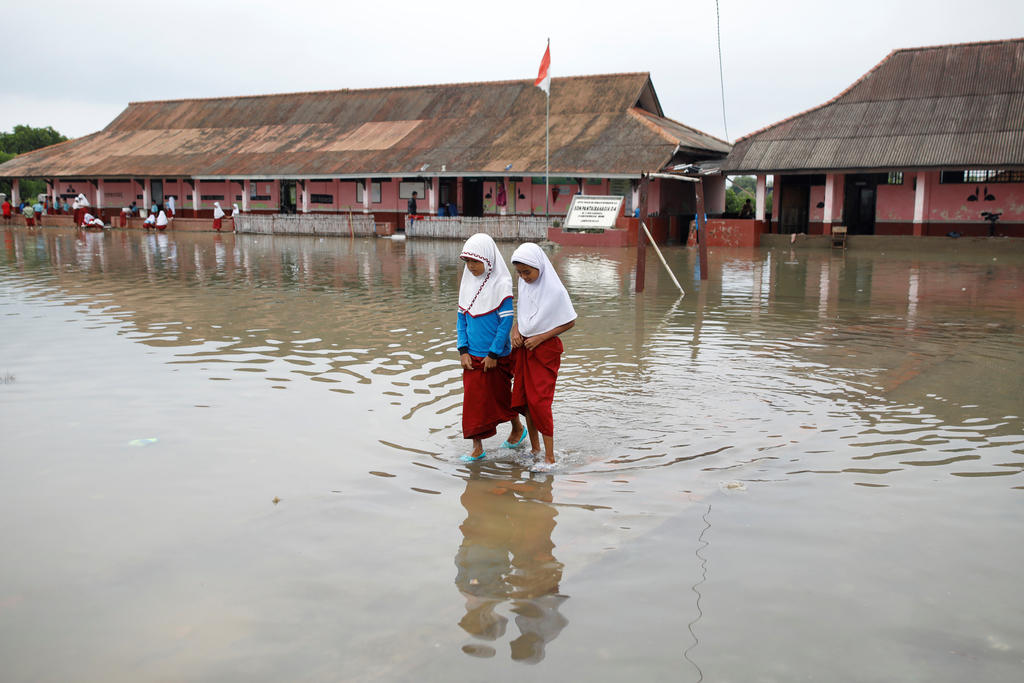
\includegraphics[width=3in]{flooded_schoolyard_indonesia.jpg}
    %\caption {Floded schoolyard in Bahagia village.}
    %\label{fig:flooded_schoolyard}
%\end{figure}


\subsection{Biotic Life in Mangroves}
\subsection{Fauna} 

\subsubsection{Mudskippers}

  Mangroves are home to a variety of animals and botic microorganisms that make them one of the most productive ecosystems in the world \citep{kristensen1991benthic}. One of the most unique organisms that inhabit this ecosystem is the mudskipper (\textit{Gobiidae: Oxudercinae}). These amphibious fish are both marine and land-faring organisms. They have evolved to maneuver through muddy landscapes using their pectoral fins for support  (figure \ref{fig:mudskipper}).. For this reason, they thrive in shallow, estuarine environments such as mangrove forests that offer a balance between intertidal and muddy zones. These small creatures are also good indicators of ecological health. They provide insight on anthropologically induced threats to estuarine quality, as factors like chemical runoff and extreme sediment deposition dwindle this environment's ability to support life and make it uninhabitable for mudskippers \citep{polgar2009species}. 

  
  \begin{figure}[!h]
    \centering
    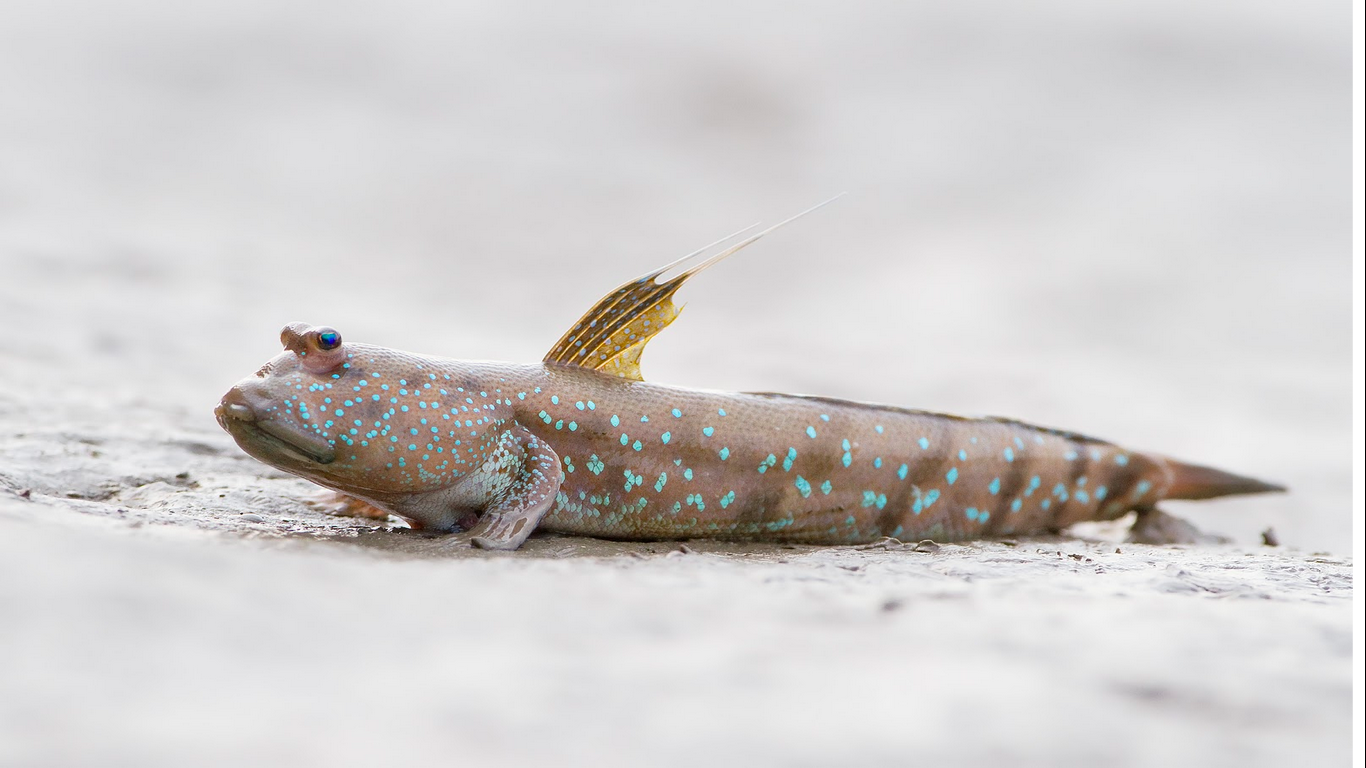
\includegraphics[width=3in]{mudskipper.png}
    \caption {Mangroves are home to a variety of animals, such as the mudskipper}
    \label{fig:mudskipper}
\end{figure}


\subsubsection{Crabs}
  Similar to mudskippers, the Grapsid crab (\textit{Crustacea: Decapoda: Grapsidae}) thrives in benthos and above water. These 4 to 6 inch shore crabs are key to recycling organic matter within the mangrove ecosystem, as they deconstruct mangrove leaves and displace sediment (this action is known as bioturbation), reducing the toxicity of organic matter and shaping the topography of the ground. Their specific niche determines the productivity of  the entire forest by influencing food chains at the final trophic level: that of decomposers. As Grapsid crabs transform organic material into digestible particulates for detritivores, they speed up the process of decomposition that cycles organic substances. Because higher levels of organic matter increase an ecosystem�s BOD, this process of organic cycling balances the constantly replenished BOD levels that can be a limiting factor for environments. Grapsid crabs not only regulate nutrients, but aid in the filtration of pollutants by breaking down toxins, as mentioned earlier \citep{lee1998ecological}.



\subsubsection{Dugong}	

Dugongs, or Phayun (pay-oon) in Thailand, are another species whose survival depends on mangrove forests. Inhabiting bay waters on the outskirts of mangrove forests, Dugong feed on seagrass and interact closely with benthos. Like bioturbulant crabs, they play a significant role in shaping the sea floor as they feed on seagrass. This sister species to the manatee (known as ``sea-cows� in western settings), is valued culturally in thai communities, who have told folk legends of this mermaid-esque mammal for generations upon generations (ref- story). However, humans continue to threaten their survival, whether it be by destroying their food supply, accidental capture while fishing, or active hunting for the black market. For these reasons, the ecologically important Dugong has garnered an endangered status. 


A common precursor of species vulnerability is the drastic depletion of food sources. In the case of Dugong, farmers are responsible for diminishing seagrass levels due to toxic fertilizer runoff.  This both kills epifaunal organisms and threatens a vital source of sustenance for the herbivorous Dugong. As for fishing, many Dugong are killed from bycatch and entanglement. Because many rural fishers lack the means to apply technologically advanced and ecologically conscious practices, they often resort to traditional, yet illegal practices. Their unintentional capture typically takes one of three forms: via gill nets, stake traps, or push nets, which scoop and trap organisms as it is scraped against the seafloor. These low tech, high capture mechanisms tend to disrupt entire ecosystems by trapping a host of organisms other than their target species /citep{hines2005community}. Even though many locals acknowledge the faults within their fishing approaches, they may be conflicted with economic barriers. For residents of �no land village� in Bang Chan, Thailand, alternative fishing is preferable yet they lack the resources or financial stability to do so.  The reality that human survival comes at the expense of environmental degradation highlights the age old conflict between prioritizing environmental versus anthropological  needs. Undoubtedly, this is a complex and difficult problem to address. For now, the solution seems to be synthesising scientific and traditional ecological knowledge (TEK) specific to locals who know their communities best %\citep{savethedugong}. 


%As rural communities begin to modernize, they are finding new ways to supplement income and positively impact their environments. For Chao mai village in Trang province, Thailand, the conservation of Dugong has spurred development and flourished their economy. Utilizing Dugong conservation as a market to attract tourists, this village has initiated the construction of roads, a port, and a hotel to accommodate visitors. Despite these efforts however, dugongs are killed regularly to supply underground markets in Singapore where they are used for medicinal purposes.


%Despite these efforts however, dugongs are killed regularly to supply underground markets in Singapore. Worth about \$2000 USD in the black market and poached at the rate of 25 Dugong per month, an estimated profit of \$600,000 USD fuels the illegal trade \citep{savethedugong}. Of course, these calculations only account for dugong within Thailand and are conservative estimates at that. Although it is difficult to prevent the supply side of this, activists are attempting to re-educate the demand side, especially those who believe dugong have medicinal benefits when consumed.
  
  Overall, dugong are very closely tied to mangroves as they exist and depend on many of the same ecological elements, hold a similar cultural value, and are threatened by human impact.


\begin{figure}[!h]
    \centering
    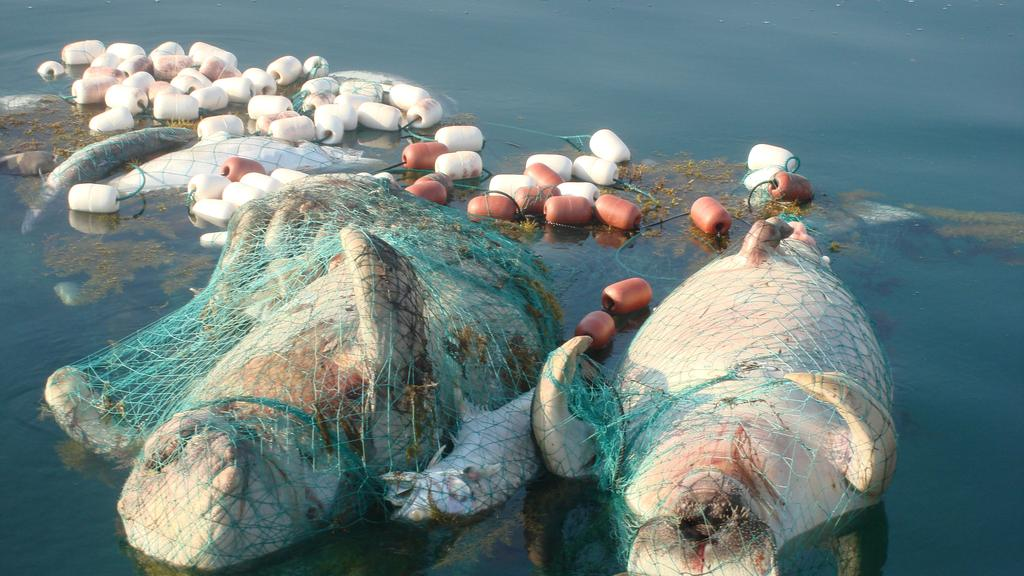
\includegraphics[width=3in]{dugongtangle.jpg}
    \caption {Endangered species: dugongs can be trapped by large gill nets and drowned.}
    \label{fig:dugongtangle}
\end{figure}


  As rural communities begin to modernize, they are finding new ways to supplement income and positively impact their environments. For Chao Mai village in Trang province, Thailand, the conservation of Dugong has spurred development and flourished their economy. Utilizing Dugong conservation as a market to attract tourists, this village has initiated the construction of roads, a port, and a hotel to accommodate visitors. 

Reading Activity: Look up other mangrove fauna and pick one that interests you and tell a friend about it!  

\subsubsection{Flora}
Mangrove forests are filled with a diverse range of plants including trees, underwater seagrass, and shrubs. Mangroves are commonly lined with Rhizophora apiculatas, or red mangrove trees, that grow in sheltered areas. Another mangrove, the Excoecaria agallocha, of the Euphorbiaceae family, is considered one of the most  economically profitable trees because of its soft wood. Additionally, mangrove forests are complimented with beds of sea grass that keep the intertidal zones rich in nutrients for the many animals living within the area. Sea grass too, has filtration properties and can mitigate coastal erosion in much the same way as mangrove trees \citep{hoegh1999climate}. 

\begin{figure}[!h]
    \centering
    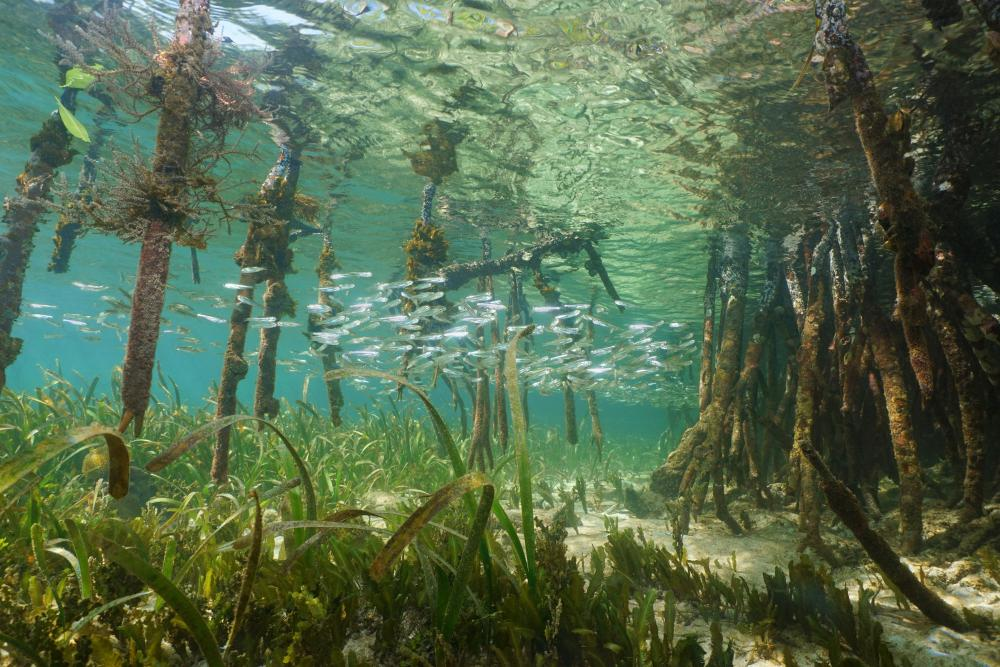
\includegraphics[width=3in]{seagrass.jpg}
    \caption {Seagrass flourishes in shallow benthic zones, and are often key organisms of mangrove ecologies.}
    \label{fig:seagrass}
\end{figure}


\subsection{Abiotic Factors}

\subsubsection{Nutrients}
While nitrogen and phosperherous are vital for Mangrove survival, mangroves rely most heavily on ammonium, a form of nitrogen within the soil. 
%\cite{doi:10.1093/treephys/tpq048}

Mangroves tend to have low levels of dissolved nutrients in the sediment and water. In result, they possess a high capacity for retaining and recycling nutrients by several mechanisms that reduce loss. Mangrove sediments are unique and have low concentrations of inorganic nitrogen, low release to the tidal water, and low rates of net transformation, and efficient microbial assimilation \citep{kristensen2000carbon}. Mangroves are highly efficient ecosystems that utilize and recycle their nutrients and provide a rich environment for flora and fauna to florish. 



\subsection{Rizospheric Bacteria in Mangroves}

\subsubsection{Bacterial Oxygen Distribution}

  As mentioned previously, mangrove forests are carbon rich due to their ability to store large amounts of organic matter. In order for this ecosystem to function properly however, the organic matter must be decomposed by aerobic bacteria in the benthic zone and rhizosphere. But because they are aerobic, these bacteria place heavy biological oxygen demands (BOD) on the environment. To mitigate this, mangroves act as oxygen highways that transport O2 down to their roots, where it then leaks and supplies surrounding bacteria. These roots can have almost atmospheric levels of O2, at impressive concentrations of 14 to 19\% \citep{scholander1955micro}. This process is much faster than the percolation alternative, in which O2 would otherwise dissolve vertically from atmospheric to rhizospheric levels. As you can imagine, this would not only be a long journey, but would diminish the oxygen concentration with each respective layer. With already limited oxygen availability in the water, even smaller amounts are able to diffuse through mud. %The rapid decrease in O2 concentration from interface to interface is modeled in fig #.
  
  Eventually these insufficient stores of O2 run out, at which point bacteria will switch to nitrogen as its main fuel. After available nitrogen levels are depleted, bacteria will begin to consume iron, sulfur, and eventually carbon dioxide. At this final level of succession in which bacteria are reliant on CO2, methane will be produced through a series of reactions, creating swamp gas. 
  
  To understand this process, refer to figure \ref{fig:oxygendiagram}. In this diagram, the efficiency of bacteria decreases with soil depth. Because oxygen diffuses at a slow rate, it is used by organisms nearest to the soil surface, while deeper bacteria are accustomed to other ions for their survival. The same can be said horizontally, in reference to root proximity. Bacteria nearest mangrove roots typically rely on O2 and are most efficient, whereas those farthest away are more likely to use nitrogen or other less productive means. As a result, natural selection dictates that organisms relying on inefficient metabolic pathways will be outcompeted, and their ability to oxidize organic carbon to CO2 and release energy will be inhibited \citep{dodds2002freshwater}. This is influential in mangrove health as oxygen deficient bacteria are weak and inefficient at breaking down organic matter, which produces a dissolved oxygen (DO) strain on other ecological organisms, like fish and shrimp. 
  
  
  \begin{figure}[!htb]
      \centering
        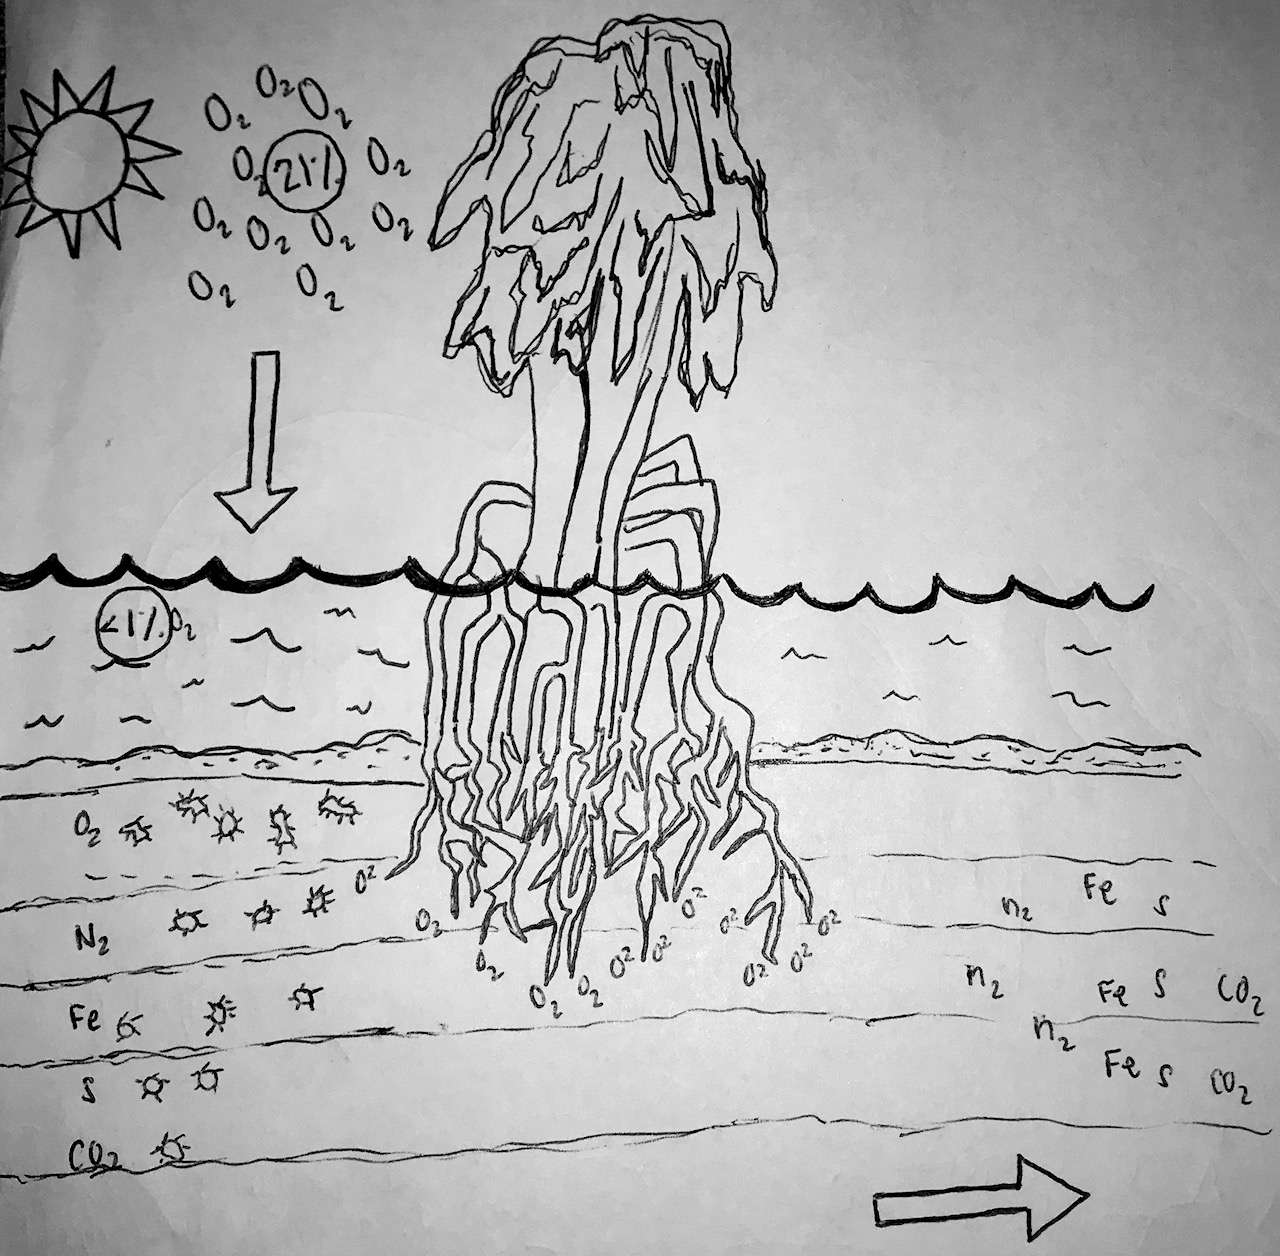
\includegraphics[width=4in]{oxygendiagram.jpg}
        \caption {Available oxygen is lost down the vertical gradient as well as further from mangrove roots.}
        \label{fig:oxygendiagram}
\end{figure}
  


\subsubsection{Root Exudates and ``Good Bacteria"}

  Microbial inoculants are microorganisms that boost plant health and nutrient uptake by warding off harmful pathogens. Serving as barriers from disease, these inoculants can be referred to as good microbes and usually take one of three forms: bacteria, fungi, or trichoderma. Existing in the rhizosphere, these helpful microbes have symbiotic, or mutually benefitting, relationships with plant roots. In particular, they work closely with root exudates, which provide them sustenance in the form of sugars, amino acids, peptides, enzymes, vitamins, organic acids, nucleotides, fungal stimulators, inhibitors and attractants, oxygen, and more \citep{shukla2011nature}. The ability for inoculants to successfully blockade harmful contaminants, let alone survive, is reliant on a constant supply of these specific chemical compounds and macronutrients. In addition, microbes are tasked with breaking down organic matter into usable nutrients like phosphorus and nitrogen that allow for tree growth. 
	
	
  Root exudates also function as signaling mechanisms that alert the rest of the tree to potentially dangerous bacteria. Typically, root exudate intervention is categorized in either positive or negative terms. An example of positive root secretion would entail chemical signaling to attract 'good bacteria', such as plant growth-promoting rhizobacteria (PGPR). Conversely, negative secretion involves the release of harmful toxins to drive out competing plant species and repel detrimental microorganisms \citep{shukla2011nature}. In doing so, root exudates inject plant-based poisons known as phytotoxins downward into the Rhizosphere \citep{shukla2011nature}. Pathogen fighting �chemical weapons�, these are delivered to the soil-root substrate with the help of unique protein transporters \citep{baetz2014root}.

	 Interestingly, this process is thought to be fueled by sulfur rather than oxygen. In much the same way as sulfate reducing bacteria, root exudates are anoxic and anaerobically transform sulfate (SO42�) into hydrogen sulfide (H2S) as they power other processes like defense transport \citep{van2002rocks}. Theses areas included vegetated zones, presumably with higher levels of tree density and biodiversity, rather than unvegetated mudflate (UN) areas.

\subsubsection{Heavy Metals}

  Besides deflecting pathogens, tree roots demobilize heavy metals from toxifying their surrounding environments. This process of preventing root absorption and soil dispersion of heavy metals is called phytostabilization. To accomplish this, roots establish a quarantine zone of sorts, that keeps contaminants spatially confined. It is important to note that phytostabilization does not absorb pollutants into plant tissue, but sequesters pollutants in soil near the roots, becoming less bio-available and reducing exposure to humans, livestock, and wildlife \citep{deBashana2012ThePC}. On the other hand, phytoextraction entails the direct uptake of toxins so long as the metabolism of the plant is resistant to its toxicity, and can still maintain its functionality \citep{mccutcheon2003overview}. While only certain toxins may qualify for phytoextraction, this is a unique biological adaptation nonetheless. Phytostabilization and phytoextraction are not mutually exclusive, and plants depend on both for their vitality. Without these processes, dangerous concentrations of heavy metals such as lead or manganese that run off from shrimp aquaculture would likely bioaccumulate in mangrove food chains. Heavy metals are especially a threat in dry seasons, where larger amounts of toxins are sediment, runoff, and organic matter deposit these toxins \citep{handayani2015migration}.  


  Overall, root exudates are a vital component not only to their respective plants, but to their surrounding environments as a whole. With the help of microbial inoculants, they are capable of bioremediation in the form of pollution decontamination and plant regeneration. As a team, these two strengthen forest productivity, density, and as a result, biodiversity. This is such an effective relationship, that studies inoculating seedlings with plant-growth-promoting bacteria have proven to be successful in facilitating reforestation \citep{bashan2008environmental}. Recently, these ecologically restorative properties have given rise to increasing rizopheric research, in which many are beginning to investigate natural biogeochemical processes as a solution to environmental degradation \citep{shukla2011nature}. 


\section{Shrimp Farming and Aquaculture}
From 1961 to 1966, the mangrove land coverage in Thailand was reduced by half of its original area \citep{naito2014relationship}.  As mangroves areas flooded with brackish water, the land became an ideal location for shrimp aquaculture. As a result of the increase of shrimp farming, 16-32\% of mangroves have been destroyed \citep{chambers2011aquaculture}. Thailand produces 550,000 tons of shrimp annually and disperses its crops around the globe. In 2005, it was discovered that shrimp farming has contributed approximately \$1.2 billion to the Thai economy. Because of the large impact and role shrimp farming plays in progressing the Thai economy, the Thai government has been accused of valuing shrimp aquaculture�s economic benefits over environmental issues \citep{trisurat2006community}. Intensive shrimp aquaculture requires artificial feed, pesticides, antibiotics and harmful chemical compounds. The components that are found in the discharge include solid matter (eroded pond soils), organic matter (rotting shrimp feed, dead shrimp, and shrimp feces), and dissolved metabolites (ammonia, urea, and carbon dioxide). Some materials, such as chemical compounds and antibiotics, are quite toxic. However, there is a lack of literature that exists proving these environmental hazards because of the strict governmental control over shrimp farming. Most shrimp farms dispose of the polluted water and waste products into surrounding areas and nearby waterways. Although shrimp farms are typically formed on lands that were previously mangrove ecosystems, mangroves still surround the areas in close proximity to today�s shrimp farms \citep{aksornkoae2004overview}. A study conducted in the mangroves in Pak Phanang province, Thailand, found  that excess sediments discharged from nearby shrimp farms flows into the nearby mangroves. The waste affected mangroves by reducing growth rates and increasing mortality rates \citep{vaiphasa2007impact}. The survival of mangroves and its biodiversity is threatened by the growing shrimp farming industry in Thailand. More environmentally-cautious procedures need to be adopted by shrimp farmers in order to sustain mangrove ecosystems. 

\begin{figure}[!htb]
      \centering
        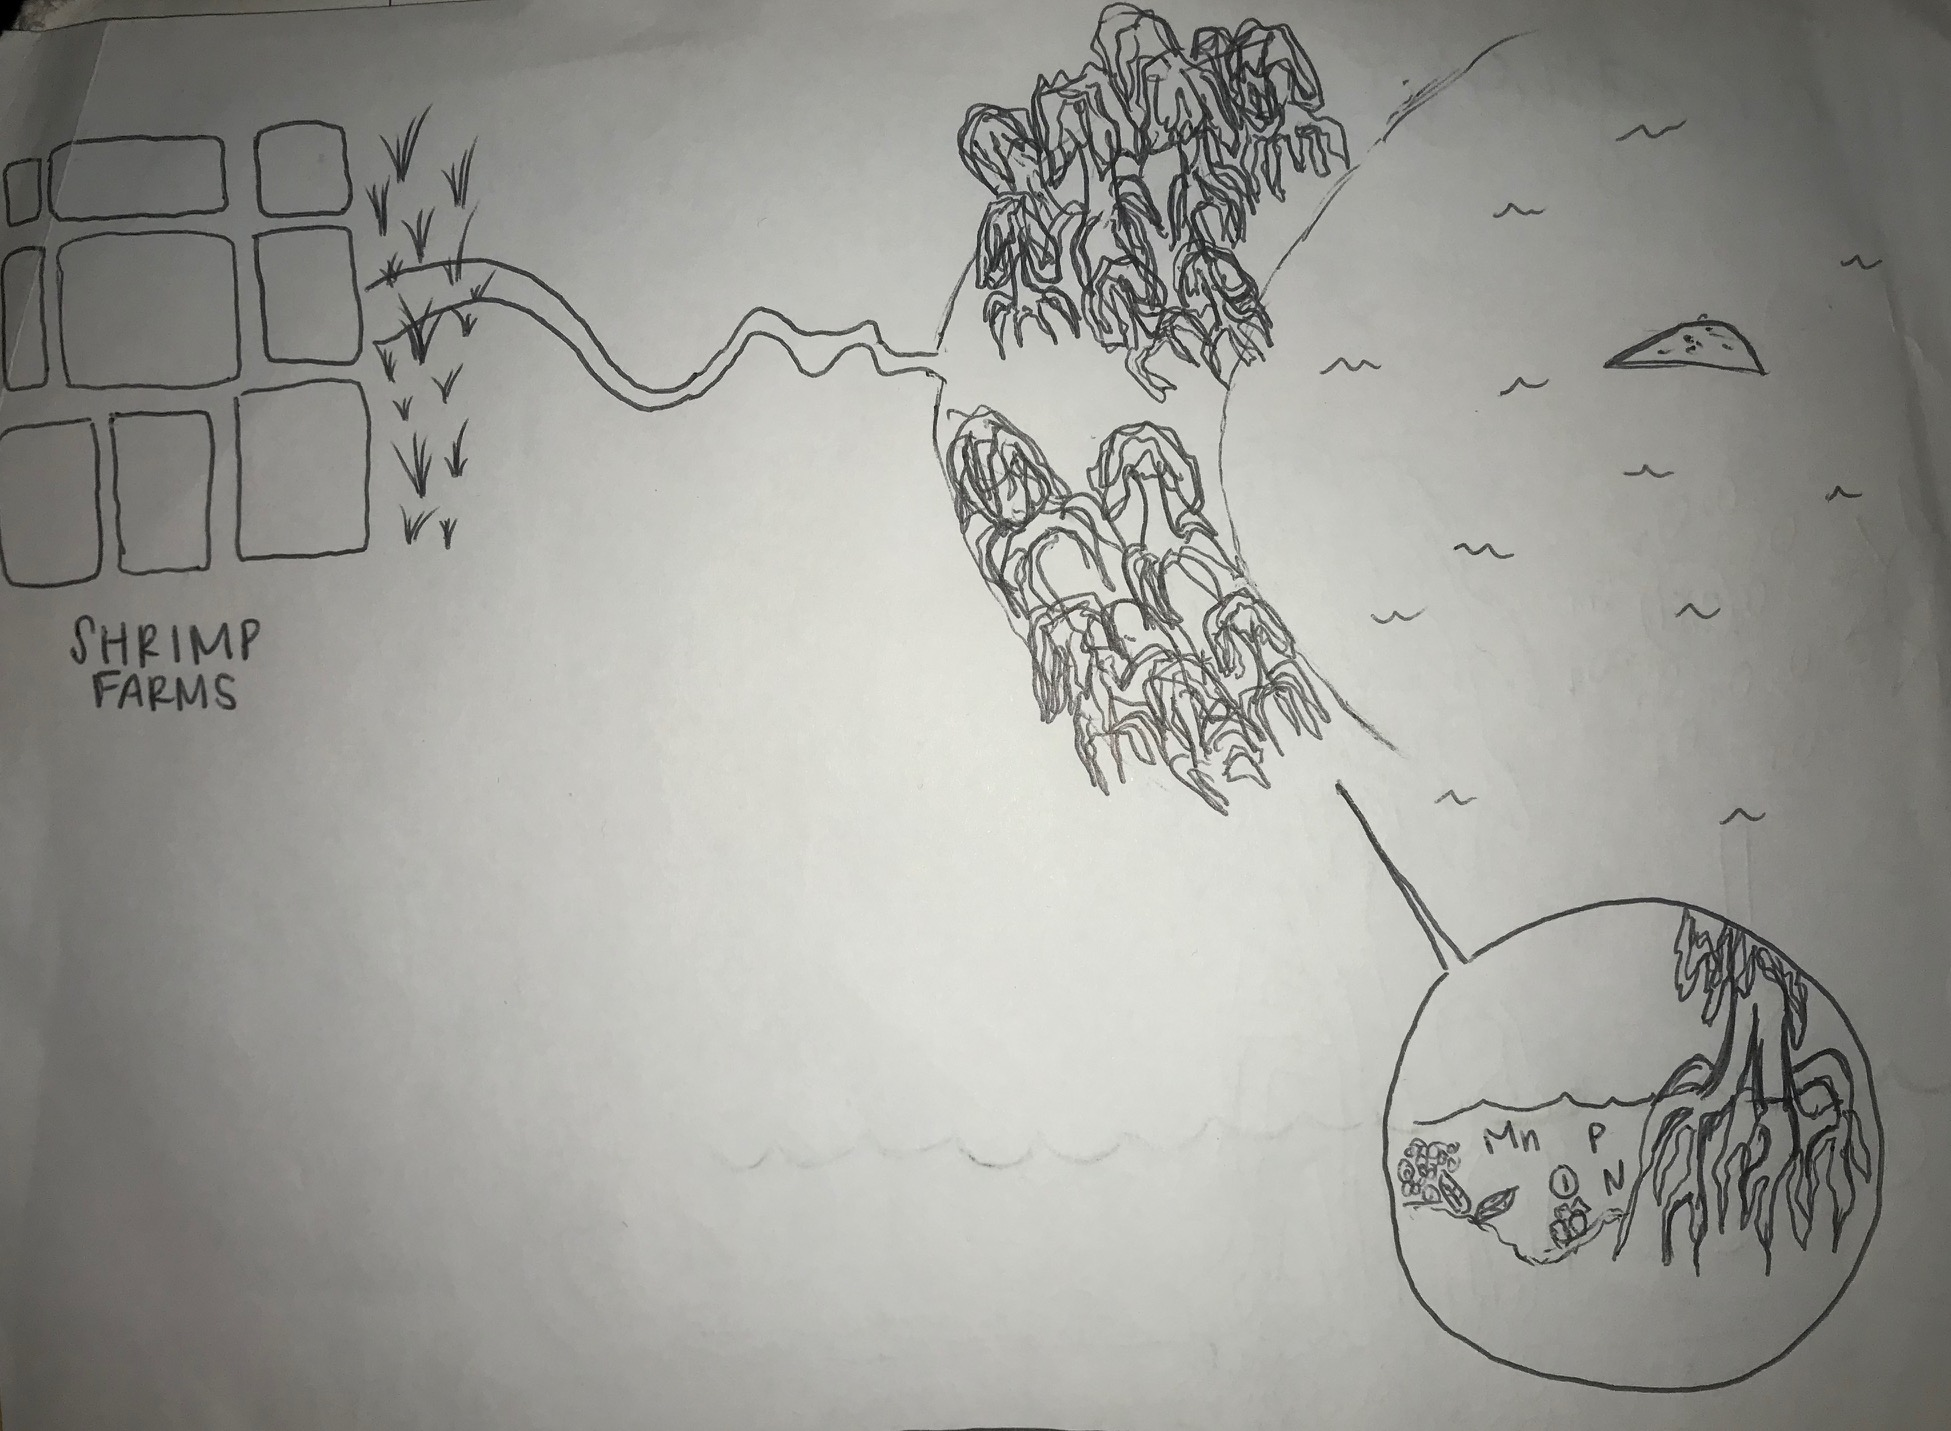
\includegraphics[width=4in]
        {shrimpdiagram.jpg}
        \caption {Chemical and nutrient runoff from shrimp farms are trapped in mangrove forests, minimizing the amount of manganese, phosphorous, nigrogen, organic material, sediment, and other phytotoxins deposited in the ocean. }
        \label{fig:shrimpdiagram}
      \end{figure}

\section{Conclusion}
The benthic water zone is a quite remarkable foundational interface that facilitates metabolic chemical processes. At the sediment-water interface, benthos facilitate sulfate reduction which results in hydrogen sulfide. Although hydrogen sulfide is toxic when present in drinking water, its ability to reduce the risk of groundwater contamination by transforming metals is environmentally useful. Benthos and benthic wayer layers in the mangroves are especially productive and diverse, supporting a large amount of biodiversity. Mangroves have a significant ecological importance and hold value in the environmentally beneficial flora and fauna. Although conservation efforts for mangrove forests have been initiated, many forests continue to be destoryed for commerical shrimp farming. The advancement and development of the shrimp farming industry in Southeast Asia has threatened the exisitence of mangrove forests and have caused environmental hazards such as pollution runoff and deforestation. Action should be taken to plan for a more sustainable future where both humans and natural organsims are able to benefit from the productivity of mangrove forests.

